\documentclass{beamer}
\usetheme{Frankfurt}
\input{commands_packages}
\graphicspath{{Figures/}}
\newcommand{\Col}{\text{Col}}
\usepackage[euler-digits]{eulervm}
\usetikzlibrary{decorations.pathreplacing,angles,quotes}

\begin{document}
\title{Clustering and Metric Space Magnitude}   
\author{Leo Selker \\ Advisor: Vin de Silva} 
\date{\today} %October 7th, 2016

\frame{\titlepage} 
\frame{\frametitle{Outline}\tableofcontents}

\section{Motivation}
\frame{\frametitle{Hierarchical Clustering}
Hierarchical clustering is a general approach to data analysis
\begin{itemize}
\item Points represent data 
\item Idea: Capture structure at various scales
\end{itemize}
\vspace{1cm}
\[
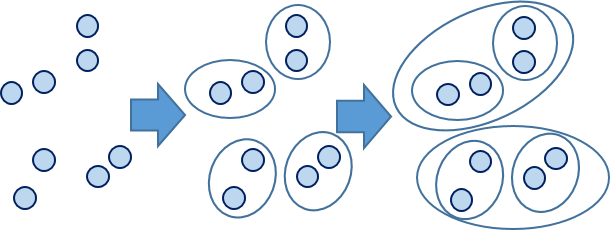
\includegraphics[width = 0.7\paperwidth] {multiscale_structure.png}
\]
}
\frame{\frametitle{Plan}
\begin{itemize}
\item There are relatively intuitive ways of clustering: We could connect points within distance $k$ of each other and then scale $k$
\item But we're exploring a weird approach
\item Very common idea: We will represent data as a \textit{finite metric space}
\end{itemize}
}2
\section{Metric Spaces}
\frame{\frametitle{Metric Spaces}
A \textbf{metric space} is a set $X$ together with a function $d: X \times X \rightarrow \Rr^{\geq 0}$, such that for all $x, y, z \in X,$
\begin{itemize}
\item $d(x, y) \geq 0$, with equality $\iff x = y$;
\item $d(x,y) = d(y,x)$; and
\item $d(x,y) + d(y,z) \geq d(x,z)$.
\end{itemize}
A metric space whose underlying set $X$ is finite is called a \textbf{finite metric space}.
\begin{itemize}
\item Useful example: Finite set of points in $\Rr^n$ (or even $\Rr^2$)
\end{itemize}
}

\iffalse
\frame{\frametitle{Data as a Metric Space}
\begin{itemize}
\item Data consists of a finite set of samples over $n$ variables
\item Very common idea: Represent data as points in $\Rr^n$. 
\item Note: $\Rr^n$ has more structure than we need. We only care about distance. \begin{itemize}
\item Any finite metric space would work
\end{itemize}
\item For any two points $x,y \in X$, let $d(x,y)$ denote the distance between $x$ and $y$. In $\Rr^n$, we'll have 
\[
d((x_1,...,x_n), (y_1,...,y_n)) = \sqrt{(x_1 - y_1)^2 + ... + (x_n - y_n)^2},
\]
which is the Euclidean distance between the two points.
\end{itemize}
}
\fi
\section{Weights}
\frame{\frametitle{Intuition Behind Weighting}
\begin{itemize}
\item We want to count the number of clusters in a space. We'll do it in a weird way:
\item[] \begin{itemize}
\item Assign a \textbf{weighting} to the points, i.e. assign each point a real-valued "weight"
\item We want each cluster's weight to sum to close to 1
\item Points near many other points will have smaller values
\item Points which are separated will have larger values
\end{itemize}
\item Then, we'll sum the weights to get the \textbf{magnitude}, i.e. number of clusters, in the data set.
\item Note: There is no "correct" or "actual" number of clusters in a space
\end{itemize}
}
\frame{\frametitle{Weighting and Magnitude}
\begin{itemize}
\item
A \textbf{weighting} on a finite metric space $X$ is a set of weights $\omega_x$ in $\Rr$ such that, for all $x \in X$:
\[
\sum_{y \in X}e^{-d(x,y)}\omega_y = 1
\]
Weights may be negative, but it's easier to think of them as nonnegative.
\item Then the \textbf{magnitude} of $X$, denoted $|X|$, is defined by:
\[
|X| = \sum_{x \in X}\omega_x.
\]
\item May be various weightings, but all lead to the same magnitude
\item Scale-dependent, which is why it's useful - see examples to come
\end{itemize}
}
\section{Examples}
\frame{\frametitle{Two Points}

Consider the space of two points separated by distance $d$:\\

                        \[
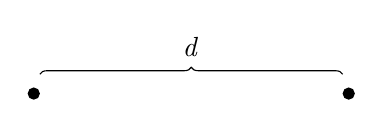
\begin{tikzpicture}[auto, node distance = 3cm, main node/.style={dot}]

\node[circle, draw, fill=black,
                        inner sep=0pt, minimum width=4pt](1) at (0,0) {};
\node[circle, draw, fill=black,
                        inner sep=0pt, minimum width=4pt](2) at (4,0) {};

\draw[decoration={brace,raise=7pt},decorate] (1) -- (2) node[midway, above = 10pt] {\textit{d}};

\end{tikzpicture}\]
\begin{itemize}
\item If $d$ is small, we expect there to be one cluster, and if $d$ is large, 2 clusters.
\item In this case, the weight of each point is equal to 
\[\frac{1}{1+e^{-d}}\]
so the magnitude is
\[
\frac{2}{1+e^{-d}}.
\]
\end{itemize}
}
\frame{\frametitle{Two Points Plot}
The space's magnitude as we scale $d$ (Note that the $x$-axis is the log of $d$):
\centerline{
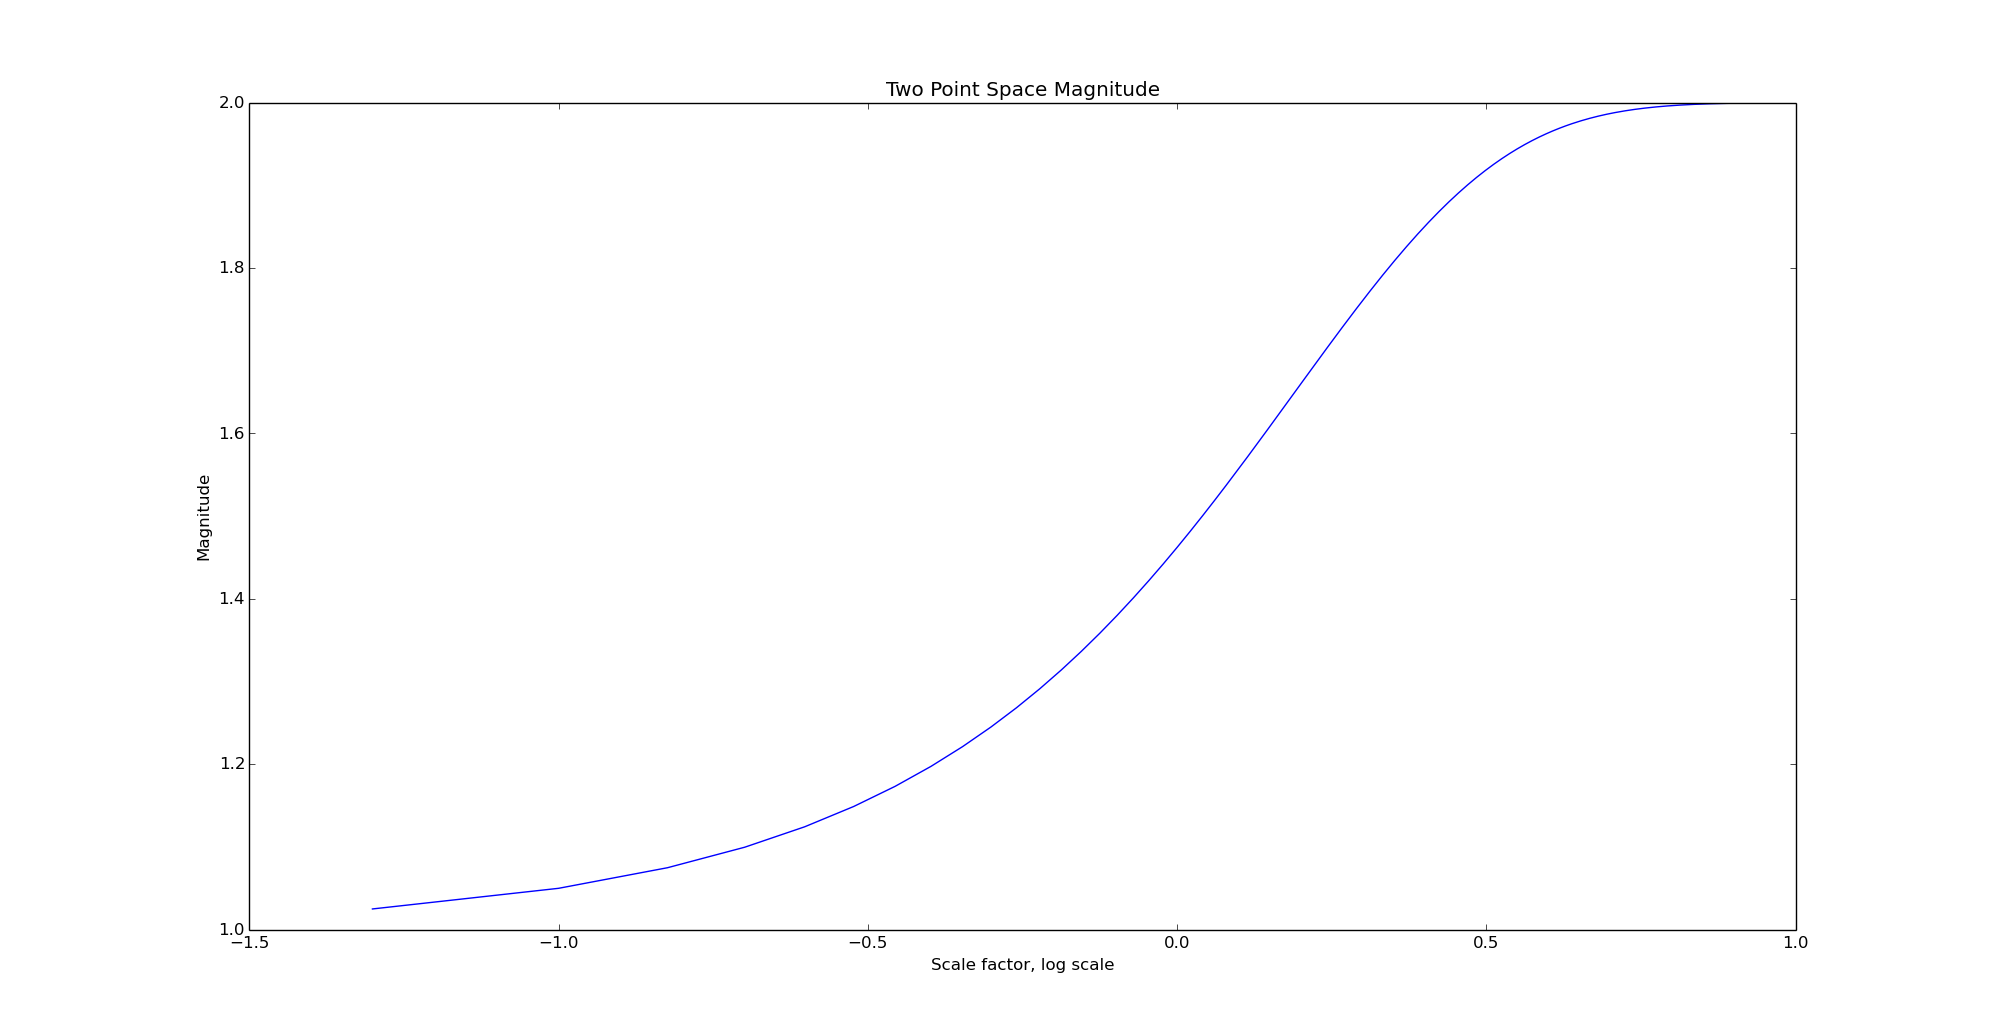
\includegraphics[width = 1.2\textwidth]{2_point.png}
}
}
\frame{\frametitle{Another Example}
Consider the space below:\\

                        \[
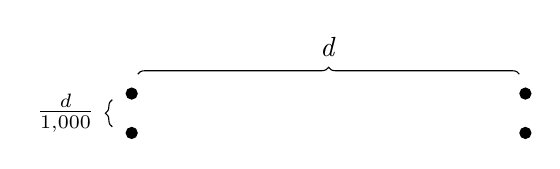
\begin{tikzpicture}[auto, node distance = 3cm, main node/.style={dot}]
\node[circle, draw, fill=black,
                        inner sep=0pt, minimum width=4pt](1) at (0,0) {};
\node[circle, draw, fill=black,
                        inner sep=0pt, minimum width=4pt](2) at (5,0) {};
\node[circle, draw, fill=black,
                        inner sep=0pt, minimum width=4pt](3) at (0,-.5) {};
\node[circle, draw, fill=black,
                        inner sep=0pt, minimum width=4pt](4) at (5,-.5) {};
\draw[decoration={brace,raise=7pt},decorate] (1) -- (2) node[midway, above = 10pt] {\textit{d}};
\draw[decoration={brace, mirror, raise = 7pt},decorate] (1) -- (3) node[midway, left = 10pt] {\textit{$\frac{d}{1,000}$}};
% \draw (2) -- (4);
% \draw (3) -- (4);
\end{tikzpicture}\]\\
\begin{itemize}
\item As we increase $d$, we would expect this to have 1 cluster, then 2, then 4
\end{itemize}
}
\frame{\frametitle{Four Points Plot}
The magnitude plot:
\centerline{
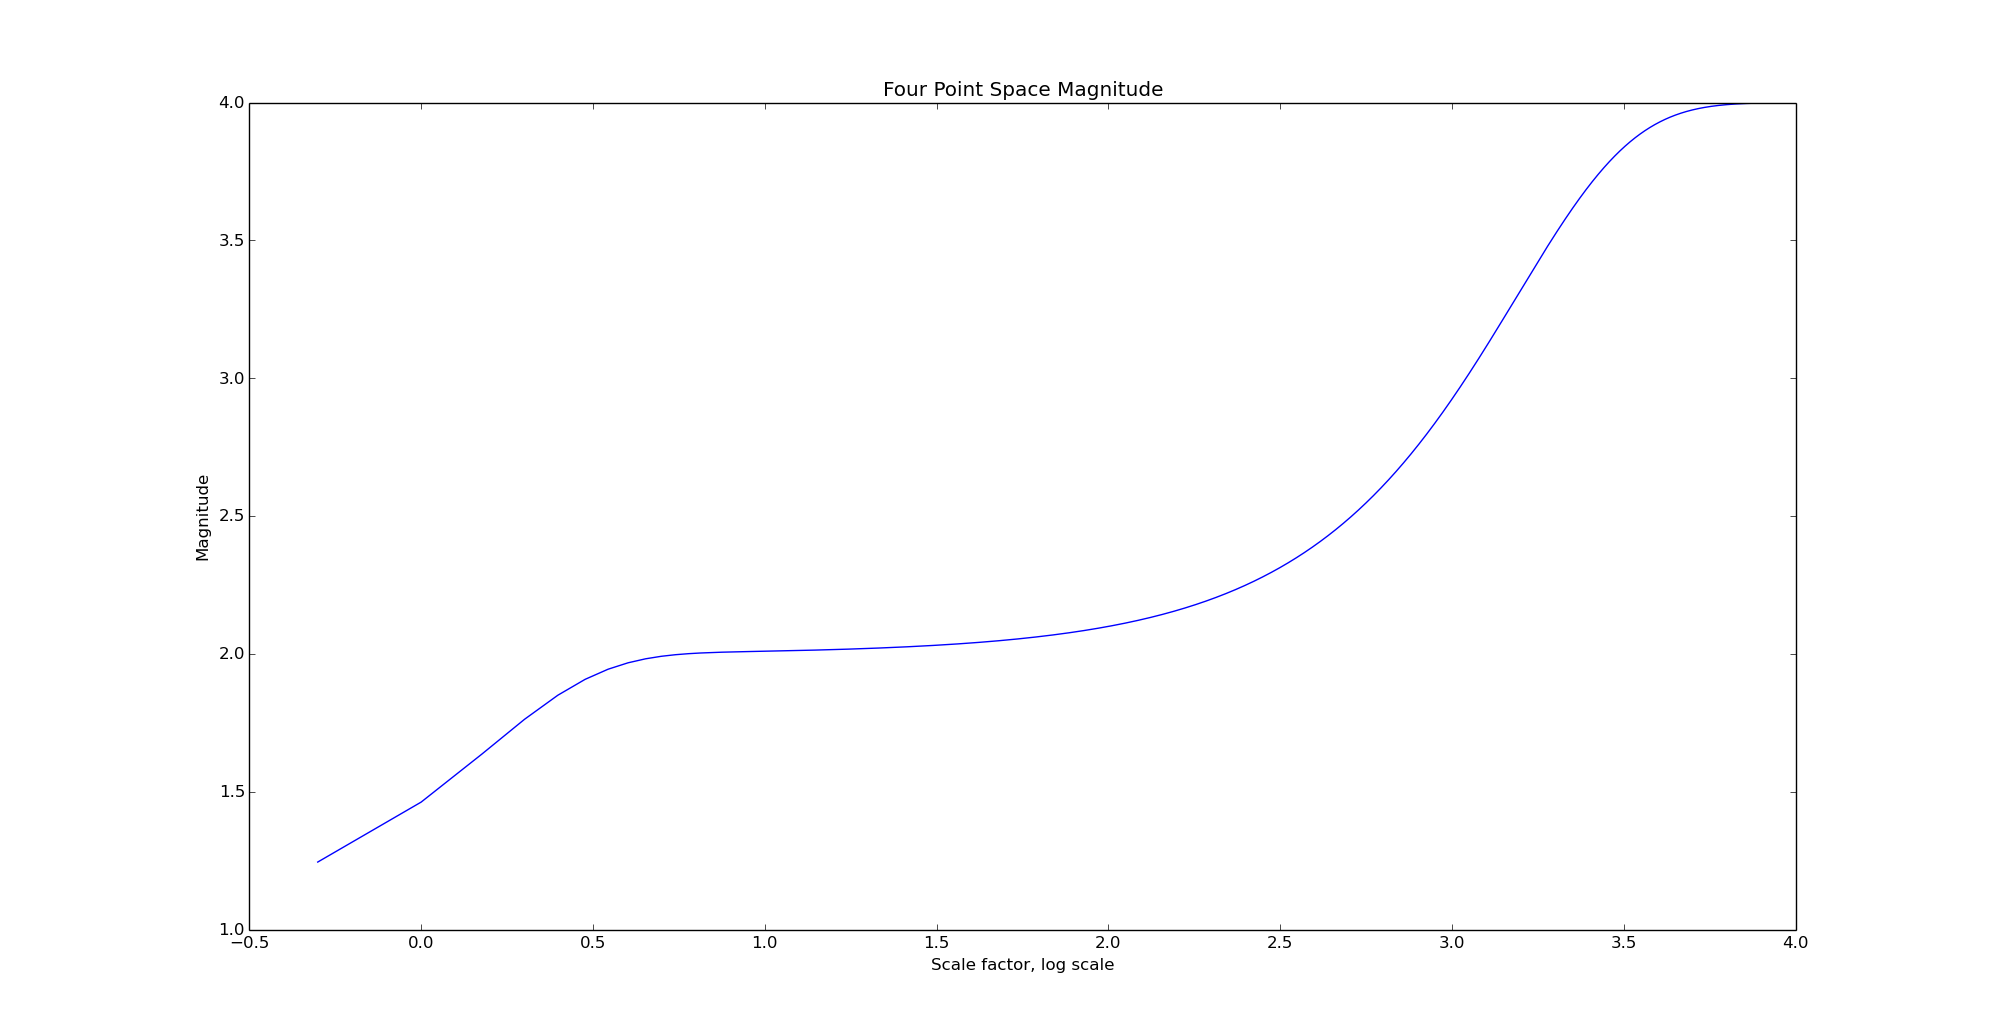
\includegraphics[width = 1.2\textwidth]{4_point.png}
}
}
\section{}


\frame{\frametitle{}
\begin{center} {\huge Thank you!}\end{center}
}

\end{document}

